\documentclass[a4paper,10pt,numbers=noendperiod]{scrartcl} 
\setlength\oddsidemargin{0.2cm}
\setlength\evensidemargin{0.2cm}
\setlength\textwidth{15.8cm}

\usepackage{amsfonts}
\usepackage{amssymb}
\usepackage{amsmath}
\usepackage{amsthm}
\usepackage{tikz}
\usepackage{wasysym}
\usepackage{ucs}
\usepackage{stmaryrd}
\usepackage{hyperref}
\usepackage{graphicx}
\usepackage{nicefrac}
\usepackage[english]{babel}
\usepackage{marvosym}
\usepackage{dsfont}
\usepackage{listings}
\usepackage[utf8x]{inputenc}
\usepackage[T1]{fontenc}
\usepackage{enumitem}
\usepackage{tabularx}
\usepackage{url}
\usepackage{eurosym}

\def\thesubsubsection{Exercise \arabic{section}.\alph{subsection}.\arabic{subsubsection}} 
\def\thesubsection{\arabic{section}.\alph{subsection} - } 
\def\thesection{\arabic{section}}



\lstset{ %
language=C++,                % the language of the code
basicstyle=\footnotesize,       % the size of the fonts that are used for the code
numbers=left,                   % where to put the line-numbers
numberstyle=\footnotesize,      % the size of the fonts that are used for the line-numbers
stepnumber=1,                   % the step between two line-numbers. If it's 1, each line 
numbersep=5pt,                  % how far the line-numbers are from the code
backgroundcolor=\color{white},  % choose the background color. You must add \usepackage{color}
showspaces=false,               % show spaces adding particular underscores
showstringspaces=false,         % underline spaces within strings
showtabs=false,                 % show tabs within strings adding particular underscores
frame=single,                   % adds a frame around the code
tabsize=2,                      % sets default tabsize to 2 spaces
captionpos=b,                   % sets the caption-position to bottom
breaklines=true,                % sets automatic line breaking
breakatwhitespace=false,        % sets if automatic breaks should only happen at whitespace
title=\lstname,                 % show the filename of files included with \lstinputlisting;
}



\author{Ralph Krimmel}
\title{xmpproxy, a proxy server for the XMPP protocol}
\subtitle{ Project description and plan }


\begin{document}
\maketitle{}
\thispagestyle{empty}
\newpage
\tableofcontents{}
\newpage

\section{Abstract}
\textit{``The extensible messaging and presence protocol xmpp is an open technology 
for real time communication which powers a wide range of applications including instant messaging, 
presence, multi-party chat, voice and video calls, collaboration, lightweight middleware, 
content syndication and generalized routing of xml data.''}   $_{\tiny http://xmpp.org/about}$ \\

Being widely used in several large communication platforms such as \texttt{Google talk},  % Todo cite
\texttt{XMPP} has become an important protocol for communication via network. This document will describe an 
issue using \texttt{XMPP}'s instant messaging capabilities in a multi client environment and propose a possible solution.
It also contains a time schedule for implementing this solution as a project for the course ``Applied IT project'' at the University 
of Gothenburg.

\section{Introduction}
The \texttt{XMPP} or ``jabber''-protocol supports multiple clients to be connected to the same account at the same time. From the server sides view a connected client is called a \textit{ressource}. The consequence of multiple ressources for the same account is that the server has to decide to which ressource an incoming message, or \textit{stanza} in xmpp terminology, is routed to. This is done via the so called \textit{presence priority} a client can connect with.  The client with the higher priority will receive the message. 
If two or more resources have the same priority, the server may use some other rule to decide between those or deliver the message to all of them. For example, the server could use the most recent connect time or the most recent activity time. However, the server is not allowed to deliver the stanza to an available resource with a negative priority. %TODO cite 

This behaviour leads to the problem, that conversations and logfiles of conversations may not be complete on every client, if one client with a higher priority connects. Figure \ref{fig:2clients} shows an example where this would be the case. Client A does not know the parts of the conversation that are held from Client B. Also, not just incoming messages will be missing, Client A will not even know about outgoing stanzas from Client B. 
\begin{figure}[h!]
	\begin{center}
		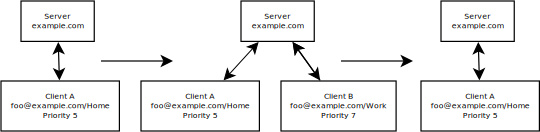
\includegraphics[scale=0.6]{figures/diagram1.pdf}
	\end{center}
	\caption{Clients with 2 different priorities are connected to the same account.}
	\label{fig:2clients}
\end{figure}


A possible solution for this issue may be the use of a proxy server as it can be seen in figure \ref{fig:2clientsproxy}. This server will make sure, that every incoming stanza will reach both clients and every outgoing stanza will be sent to every ressource as well as to the targeted server.

\begin{figure}[h!]
	\begin{center}
		
\includegraphics[scale=0.5]{figures/diagram3.pdf}
	\end{center}
	\caption{Two clients connected to a proxy.}
	\label{fig:2clientsproxy}
\end{figure}

\section{Technology}

\section{Literature}
\begin{itemize}
	\item \texttt{Programming jabber - extending XML messaging} by DJ Adams\\
	\item \url{http://xmpp.org/rfcs/rfc6120.html}\\
	\item \url{http://xmpp.org/rfcs/rfc6121.html}\\
	\item \url{http://xmpp.org/rfcs/rfc6122.html}\\
	\item \url{http://search.cpan.org/~hacker/Net-XMPP-1.02/}\\
	\item \url{http://search.cpan.org/~mart/DJabberd-0.85/}\\
\end{itemize}


\section{Schedule}
\end{document} 
